\chapter{Introduzione alla sicurezza informatica}


\section{Premessa}

\subsubsection{Definizione}
Che cosa significa sicuro? La parola sicurezza e l'aggettivo sicuro vengono sempre associati a beni che si desidera proteggere da possibili danni, perdita, accessi non consentiti e via dicendo. In particolare un bene è al sicuro se è ben protetto, e \textbf{la sua messa in sicurezza non ne impedisce l'utilizzo}. Esistono molteplici definizioni di sicurezza informatica, ad esempio:
\begin{itemize} 
  \item Security is the degree of protection against danger, damage, loss, and criminal activity 
  \item Security is a form of protection where a separation is created between the assets and the threat 
\end{itemize}
La parola sicurezza deriva dal latino \textbf{sine cura}: senza preoccupazione. La sicurezza di un sistema può essere definita come la conoscenza del fatto che l'evoluzione del sistema stesso non produrrà stati indesiderati. Le cause che possono minare la sicurezza sono molteplici e spesso non prevedibili, quindi non si può parlare di sicurezza in senso assoluto, ma solo relativo (\textit{"L'unico computer sicuro è un computer spento"}).

\subsubsection{Trasversalità della tematica}
Le problematiche di sicurezza interessano molteplici campi (attività lavorative, vita domestica, hobby, giochi, sport, etc.). Di fatto, ogni settore della vita moderna ha delle implicazioni relative alla sicurezza. Il livello di sicurezza di un'organizzazione dipende dai livelli di sicurezza di tutti i suoi comparti/settori. Il livello di sicurezza di un sistema è determinato dal livello di sicurezza dal suo comparto meno sicuro (principio dell'anello debole).


\section{Concetti fondamentali}

\subsubsection{Sistema informativo e informatico}

\begin{itemize} 
  \item Per \textbf{sistema informativo} (information system) di un'organizzazione si intende l'insieme delle informazioni prodotte ed elaborate e delle risorse umane, materiali e immateriali, coinvolte nel processo di elaborazione di tali informazioni
  \item Per \textbf{sistema informatico} (information and communication technology system) s'intende l'insieme delle varie tecnologie coinvolte nel sistema informativo (il sistema informatico è parte del sistema informativo).
\end{itemize}
Questo corso verterà sulla sicurezza dei sistemi informativi. Tuttavia, si approfondiranno maggiormente questioni inerenti la sicurezza
dei sistemi informatici. Per sicurezza di un sistema informativo si intende il grado di protezione contro qualsiasi minaccia ai suoi asset.
Richiede il soddisfacimento dei seguenti requisiti:
\begin{itemize} 
  \item \textbf{confidenzialità, integrità e disponibilità}
  \item \textbf{assicurazione, autenticità e anonimato}
\end{itemize}
Quando si parla di \textbf{attacco} solitamente si intende la violazione di uno o più di questi requisiti.

\subsection{Vulnerabilità, Minacce, Attacchi, Difesa}
\subsubsection{Vulnerabilità}
Una vulnerabilità (o falla o breccia) è una \textbf{debolezza intrinseca} di un sistema, che potrebbe essere sfruttata per provocare perdite o danni. Scaturisce spesso da errate procedure di sicurezza e/o da errori di progettazione/implementazione, e  in alcuni casi è intimamente legata alla natura del sistema. Ad esempio:
\begin{itemize} 
  \item un sistema potrebbe essere vulnerabile alla manipolazione non autorizzata dei dati a causa di un bug nella procedura di autenticazione dell'utente
  \item un calcolatore è vulnerabile all'acqua
\end{itemize}
Nel primo caso (vulnerabilità scaturite da errate procedure di sicurezza) l'insorgenza delle vulnerabilità può essere mitigata adottando adeguati standard e norme di qualità.

\subsubsection{Minacce (Threats)}
Per minaccia (threat) ad un sistema informatico/informativo si intende quell'insieme di circostanze che potrebbero arrecare danni ai suoi asset: eventi potenziali, accidentali o deliberati, che, nel caso accadessero, produrrebbero perdite e danni. Il realizzarsi di una minaccia generalmente avviene sfruttando una o più vulnerabilità del sistema.  Si parla quindi di situazioni ipotetiche che potrebbero avvenire in determinate circostanze. Ad esempio:
\begin{itemize} 
  \item esecuzione di codice malevolo che invia dati sensibili ad un'organizzazione criminale
  \item accesso a dati riservati da parte di entità non autorizzate
  \item perdita di dati a causa della rottura di un apparato hardware o al crash di uno specifico software
\end{itemize}

\subsubsection{Attacchi (Attacks)}
Un attacco (attack) è un atto deliberato teso ad arrecare un danno al sistema. Consiste, di fatto, nella realizzazione di una \textbf{minaccia}. Generalmente, un attacco viene perpetrato attraverso lo sfruttamento di una o più vulnerabilità. Spesso si classificano in base all’entità del danno:
\begin{itemize} 
  \item \textbf{attacco attivo (active attack)}: altera le risorse o ne modifica il processo di gestione/elaborazione
  \item \textbf{attacco passivo (passive attack)}: ottiene le informazioni/dati senza alterarli e senza modificare il relativo processo di
gestione/elaborazione
\end{itemize}
Un’altra importante classificazione è in base "al luogo" da cui viene iniziato l’attacco:
\begin{itemize} 
  \item \textbf{attacco dall'interno (inside attack)}: attacco iniziato da un'entità all'interno del perimetro di sicurezza di un sistema informativo di una data organizzazione
  \item \textbf{attacco dall'esterno (outside attack)}: attacco iniziato da un'entità all'esterno del perimetro di sicurezza
\end{itemize}
Ovviamente, è molto più difficile prevenire e rilevare gli attacchi interni di quelli esterni. Ciò anche a causa del fatto che le misure di prevenzione per questo tipo di attacchi limita notevolmente l'usabilità del sistema (si pensi, ad esempio, alla struttura gerarchica in ambiente militare, in cui ogni risorsa conosce il minimo indispensabile per svolgere i propri compiti. In questo modo nel caso la risorsa venga compromessa, si limita il danno. Ovviamente tutto ciò rallenta il processo di funzionamento del sistema).

\subsubsection{Tecniche di difesa}
Diverse contromisure (o misure protettive) possono essere attuate per proteggere un sistema informativo da eventi accidentali e da
attacchi deliberati. Tali misure devono essere strutturate all'interno di un piano di sicurezza redatto dopo un'attenta analisi costi/benefici (\textit{cost-effective solutions}).
Le tecniche di difesa possono essere di tipo:
\begin{itemize} 
  \item \textbf{preventivo}: effettuano una serie di \textbf{controlli} per evitare \textbf{a priori} che attacchi noti o immaginabili possano essere sferrati con successo (e.g. controlli aeroportuali, controllo di accessi e permessi negli OS).
  \item \textbf{a posteriori}: sono tese a ridurre gli effetti di un attacco che è riuscito a eludere le misure preventive di cui sopra; devono monitorare un sistema ed essere in grado di \textbf{rivelare} comportamenti anomali.
\end{itemize}

Un \textbf{meccanismo di sicurezza} è un qualsiasi metodo, strumento, o procedura teso a rilevare, prevenire o porre rimedio agli effetti di un attacco alla sicurezza del sistema. La strategia di difesa, qualunque essa sia, combina in modo opportuno uno o più meccanismi di sicurezza (consistono in controlli hardware/software).

\subsection{Sicurezza informatica: definizione classica e requisiti CIA}
La sicurezza informatica si fonda sulla protezione dei seguenti macro-requisiti di un sistema informativo (informatico):
\begin{itemize} 
  \item \textbf{Confidenzialità (Confidentiality)}
  \item \textbf{Integrità (Integrity)}
  \item \textbf{Disponibilità (Availability)}
\end{itemize}
Spesso si utilizza l'acronimo C.I.A. per denotarli in modo compatto.
\begin{figure}[htbp]
	\centering%
	\subfigure%
	{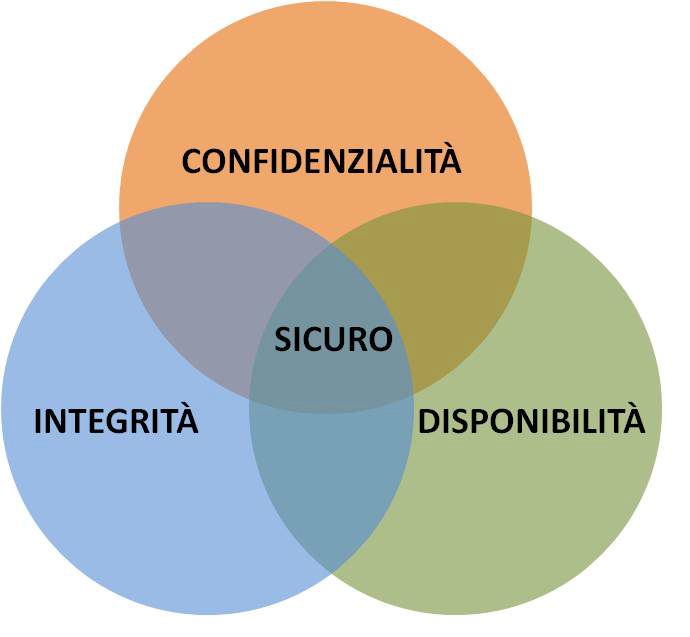
\includegraphics[height=7cm, width=7cm, keepaspectratio]{Immagini/introduzione/venn_security}}
	\caption{Diagramma di Venn dei macro-requisiti di sicurezza \label{fig:venn_security}} 	
\end{figure}
Ovviamente, come si può notare dal diagramma di Venn in \figurename~\ref{fig:venn_security}, spesso si richiede che più d'uno di questi requisiti vengano rispettati contemporaneamente, cosi come un attacco può violarne più di uno.

\subsubsection{Confidenzialità (Confidentiality)}
\textbf{Def.}: \textit{the property that information is not made available or disclosed to unauthorized individuals, entities, or processes.} \\

Per confidenzialità si intende quindi la garanzia che alle risorse informatiche accedano solo le parti autorizzate ad accedervi. E' talvolta denominata segretezza, riservatezza o privacy. Nota bene: per accesso non si intende solo la lettura, ma anche la visualizzazione, la stampa o \textbf{la semplice consapevolezza dell'esistenza di una data risorsa nel sistema}.

\paragraph{Attacchi e meccanismi di sicurezza}
Si ha un attacco alla confidenzialità quando una entità (persona, processo o risorsa) tenta di accedere senza autorizzazione a informazioni protette (mentre queste sono memorizzate, oppure durante l'elaborazione, oppure ancora durante una comunicazione). La protezione della confidenzialità avviene utilizzando in modo appropriato i seguenti strumenti (meccanismi) di sicurezza informatica:
\begin{itemize} 
  \item \textbf{Cifratura (Encryption)}
  \item \textbf{Controllo degli accessi (Access Control)}
  \item \textbf{Sicurezza fisica (Physical security)}
\end{itemize}

\subsubsection{Integrità (Integrity)}
\textbf{Def. 1}: \textit{safeguarding the accuracy and completeness of information and processing methods.}\newline
\textbf{Def. 2}: \textit{the property of safeguarding the accuracy and completeness of assets.}\newline


Per integrità si intende quindi la garanzia che le risorse possano essere modificate solo dalle parti autorizzate e solo nei modi prestabiliti. Le modifiche comprendono la scrittura, la variazione, il cambiamento dello stato, l'eliminazione e la creazione. Nel caso di file, conviene includere anche i metadati associati (proprietario, ultimo utente ad averlo letto, data ultima modifica, data di creazione), in modo che un accesso non autorizzato al contenuto possa essere rivelato da un controllo di integrità applicato ai metadati.

\paragraph{Attacchi e meccanismi di sicurezza}
Si ha un attacco all'integrità quando una entità (persona, processo o risorsa) tenta di modificare senza autorizzazione una o più risorse del sistema informativo.

 La protezione dell'integrità avviene utilizzando in modo appropriato i seguenti strumenti (meccanismi) di sicurezza informatica (tutti basati su un uso corretto della ridondanza):
\begin{itemize} 
  \item \textbf{Backup}
  \item \textbf{Somma di controllo o Checksum}
  \item \textbf{Codici a correzione di errore (Corruzioni non deliberate ma accidentali, possono essere facilmente elusi da attacchi intelligenti)}
  \item \textbf{Codici di autenticazione dei messaggi o Message Authentication Code (MAC)} 
\end{itemize}


\subsubsection{Disponibilità (Availability)}
\textbf{Def.}:\textit{ ensuring that authorized users have access to information and associated assets when required.} \newline

Per disponibilità si intende quindi che le risorse siano accessibili, nei tempi e nei modi prestabiliti, alle parti autorizzate ogni volta che le richiedono: se una persona o un sistema dispone dei diritti di accesso ad una risorsa, l'accesso non deve essergli impedito. Spesso la disponibilità viene citata tramite il suo opposto: la \textbf{negazione di servizio} (\textbf{Denial of Service} o \textbf{DoS}). La disponibilità può assumere significati/sfumature diverse: una risorsa può trovarsi in uno stato intermedio tra i due opposti stati di piena disponibilità e di piena indisponibilità.

\paragraph{Attacchi e meccanismi di sicurezza}
La protezione della disponibilità avviene utilizzando in modo appropriato i seguenti strumenti (meccanismi) di sicurezza:
\begin{itemize}
	\item \textbf{Protezioni fisiche (Physical protections)}
	\item \textbf{Ridondanze computazionali (Computational redundancies)}
\end{itemize} 

\subsubsection{Conflittualità requisiti CIA}
Spesso i requisiti di confidenzialità, integrità e disponibilità possono essere in conflitto tra loro. E' quindi importante trovare il compromesso ottimo per la garanzia di tutti e tre. E' facile garantire la confidenzialità di una risorsa impedendo a chiunque di accedervi (e.g. se chiudo la risorsa in un blocco di cemento, sicuramente resterà confidenziale. Tuttavia la disponibilità della stessa verrebbe compromessa in senso assoluto).

\subsection{Requisiti AAA}
In aggiunta ai concetti CIA, sovente viene richiesto il soddisfacimento di ulteriori requisiti che vanno sotto l'acronimo A.A.A.

\subsubsection{Assicurazione (Assurance)}
Per assicurazione si intende la corretta gestione della fiducia reciproca tra le varie parti coinvolte nell'utilizzo del sistema informativo. Tale requisito sopperisce la mancanza di regolamentazione, da parte dei requisiti C.I.A., dell'\textbf{uso delle risorse di un sistema}. E' teso quindi ad evitare un uso non consono dei vari asset del sistema. Tale concetto è ovviamente bidirezionale: così come il sistema deve fidarsi degli utenti (del fatto che non lo usino in modo inappropriato), gli utenti devono fidarsi del sistema (e.g. trattamento dei dati personali). Il concetto di fiducia è tuttavia difficile da quantificare ed è legato al grado di confidenza sul comportamento che ci si attende dal sistema. Il requisito di assicurazione viene regolato agendo sui seguenti strumenti:
\begin{itemize} 
  \item \textbf{Politiche (Policies):} specifiche comportamentali che regolano l’operato degli attori del sistema
  \item \textbf{Permessi (Permissions):} descrivono le operazioni ammesse/concesse e quelle proibite
  \item \textbf{Protezioni (Protections):} implementazione dei meccanismi di sicurezza tesi ad applicare e far rispettare le politiche e i permessi di cui sopra
  \item \textbf{Qualità del software:} lo sviluppo del software che rispetta standard di qualità rigorosi rende più difficile che il sistema si discosti dai comportamenti attesi 
\end{itemize}

\subsubsection{Autenticità (Authenticity)}
L'autenticità è la capacità di provare che dichiarazioni, politiche e autorizzazioni rilasciate da persone o sistemi siano veritiere. Se non è garantita, persone/sistemi possono sostenere argomentazioni non vere senza essere contraddetti da prove oggettive. Se è garantita, si dice anche che è soddisfatto il requisito del \textbf{non-ripudio (non-ripudiation)}. Per non-ripudio si intende che dichiarazioni autentiche rilasciate da persone e/o sistemi NON possono essere negate. La firma digitale è il principale meccanismo crittografico che permette di ottenerlo. Un contesto in cui tale requisito è importante è, ad esempio, la Posta Elettronica Certificata (PEC).

\subsubsection{Anonimato (Anonymity)}
Per anonimato si intende che non è possibile ottenere o risalire all'identità di un individuo pur avendo accesso a determinati record/transazioni di un sistema informativo. Se un'organizzazione deve rendere pubblici alcuni dati dei suoi clienti/membri senza violarne la privacy, può adottare alcuni dei seguenti strumenti:
\begin{itemize} 
  \item \textbf{Aggregazione (Aggregation):} combinare mediante somme e/o medie i dati di diversi individui
  \item \textbf{Miscelazione (Mixing):} permutare i dati dei singoli utenti in modo da preservare l'esito di predeterminate query
  \item \textbf{Mediazione (Proxies):} utilizzare degli agenti fidati che si interpongono tra l'individuo e i sistemi con i quali interagisce
  \item \textbf{Pseudonimi (Pseudonyms):} utilizzare delle identità fittizie eventualmente autenticate da una terza entità che funge da garante 
\end{itemize}

\subsection{Tipologie di Minacce e Attacchi}
E' possibile classificare diverse minacce e attacchi rispetto a quali requisiti violano. Vediamone alcune:

\subsubsection{Intercettazione (Eavesdropping)}
Si ha un'intercettazione quando un'entità non autorizzata ha ottenuto l'accesso ad una risorsa. Generalmente questo tipo di attacchi avviene nella fase di trasmissione dell'informazione, e rappresenta una violazione alla \textbf{confidenzialità}. Esempi:
\begin{itemize} 
  \item copia illecita di file di programma o dati
  \item intercettazione di una comunicazione telefonica
  \item sniffing di pacchetti di dati
\end{itemize}
Un'intercettazione potrebbe essere molto difficile da rilevare, poiché un intercettatore "silenzioso" potrebbe essere molto abile e non lasciare tracce o cancellarle. 

\subsubsection{Alterazione (Alteration)}
Si ha una alterazione o modifica quando un'entità non autorizzata, oltre ad accedere a una risorsa, interferisce con essa modificandola. Rappresenta una violazione dell'\textbf{integrità}. Esempi:
\begin{itemize} 
  \item attacchi di tipo \textbf{man-in-the-middle}: un flusso di dati viene intercettato, modificato e ritrasmesso (rappresenta anche una minaccia alla \textbf{confidenzialità})
  \item virus informatici che modificano file di sistema critici in modo da eseguire azioni maliziose
  \item alterazione dei valori di un database o modifica di un programma in modo che esegua dei calcoli diversi da quelli previsti
\end{itemize}
Alcuni casi di alterazione possono essere facilmente rilevati, mentre altre modifiche, più sottili, possono essere estremamente difficili da individuare.

\subsubsection{Interruzione (Denial-of-service)}
In un'interruzione, una risorsa del sistema viene degradata o eliminata, diventando non disponibile o inutilizzabile. Rappresenta una minaccia alla \textbf{disponibilità} e/o all'\textbf{integrità}. Esempi:
\begin{itemize} 
  \item la distruzione o il sabotaggio di un dispositivo
  \item la cancellazione di un file
  \item la congestione di un Web server causata da un numero enorme di richieste artificiali
\end{itemize}

\subsubsection{Falsificazione (Masquerading)}
La falsificazione consiste nella contraffazione di risorse (dati/hardware) da parti non autorizzate. Costituisce principalmente una violazione di \textbf{autenticità}, e a volte anche alla \textbf{confidenzialità} e/o all'\textbf{integrità}. Esempi:
\begin{itemize} 
  \item \textbf{phishing}: creazione di siti Web apparentemente identici agli originali allo scopo di frodarne gli utenti
  \item \textbf{spoofing}: spedizione di pacchetti dati con falsi indirizzi di ritorno
\end{itemize}
A volte le falsificazioni sono facilmente rilevabili, ma se attuate con abilità potrebbero essere del tutto indistinguibili da normali operazioni reali legittime.

\subsubsection{Ripudio (Ripudiation)}
Il ripudio consiste nel negare di aver effettuato una data azione. L'azione potrebbe essere la ricezione o la spedizione di un messaggio, così come l'esecuzione di una transazione. Spesso, riguarda il tentativo di recedere da un contratto (accordo) precedentemente assunto in cui era comunque previsto l'uso di ricevute (o simili) per dimostrare l'esecuzione di determinate operazioni. Si tratta di un attacco all'\textbf{assicurazione}.

\subsubsection{Inferenza (Inference), Correlation and traceback}
Per inferenza o attacco inferenziale si intendono un insieme di tecniche che, utilizzando la statistica e l'algebra, permettono di ricavare/stimare \textbf{informazioni sensibili} a partire da dati non sensibili. Rappresenta un attacco alla \textbf{confidenzialità}, e spesso è attuato nel contesto dei database. Similmente, per correlation and traceback si intendono un insieme di tecniche basate sulla statistica e sull'algebra che permettono di determinare la sorgente di una particolare informazione o di un particolare flusso di dati.\newline \newline
\textbf{N.B.:} C'è una differenza, in senso giuridico, tra dati personali e dati sensibili. Tale distinzione dipende dalla giurisdizione dei paesi. In particolare in Italia il dato personale viene indicato come un'informazione che permette di identificare un individuo (anagrafica), mentre un dato sensibile rappresenta un'informazione su aspetti della vita privata dell'individuo (orientamento sessuale, opinione politica, credo religioso, etc.).

\subsection{Principi della Sicurezza Informatica}

\subsubsection{Economia del meccanismo (Economy of mechanism)}
Il progetto e l'implementazione delle misure di sicurezza deve basarsi su modelli semplici, chiari e di facile attuazione garantendo un elevato livello di usabilità del sistema.

\subsubsection{Default sicuri (Fail-safe defaults)}
I valori di default dei modelli di controllo degli accessi e delle varie configurazioni di sistema vanno fissati in modo da garantire un buon livello di sicurezza.

\subsubsection{Mediazione completa (Complete mediation)} 
Ogni accesso ad una risorsa deve essere controllato verificando che sia conforme alle politiche di sicurezza stabilite; diffidare di miglioramenti nell'efficienza ottenuti salvando autorizzazioni precedentemente acquisite, poiché i permessi possono variare nel tempo.

\subsubsection{Struttura aperta (Open design)} 
\label{sec:openStruct}  
L'architettura, il progetto e l'implementazione dei meccanismi di sicurezza di un sistema devono essere resi pubblici. Un meccanismo di protezione ritenuto sicuro da molti è preferibile ad uno noto solo a pochi in quanto maggiori feedback favoriscono l'individuazione di bug, falle e vulnerabilità, aumentando di conseguenza la robustezza e la sicurezza del sistema. Ottenere la sicurezza dalla segretezza (\textbf{security by obscurity}) è quindi assolutamente da \textbf{evitare}, considerando inoltre che mantenere la segretezza è difficile: tecniche di reverse engineering permettono, infatti, di risalire al codice. In conclusione quindi la sicurezza deve fondarsi sulla segretezza di pochi elementi chiave, all'interno di una struttura aperta.

\subsubsection{Separazione dei privilegi (Separation of privilege)} 
Più condizioni dovrebbero essere richieste per concedere l'accesso a risorse limitate o ottenere il permesso di effettuare una data azione. In genere questo principio comporta una separazione logico/funzionale delle componenti di un sistema.

\subsubsection{Minimo privilegio (Least privilege)} 
Ogni parte di un sistema deve avere i privilegi minimi necessari allo svolgimento dei propri compiti. Per attività inusuali che richiedono maggiori privilegi conviene assegnare autorizzazioni temporanee fortemente limitate nel tempo. In questo modo si riduce il rischio di attacchi basati sulla scalata di privilegi.

\subsubsection{Minimo meccanismo comune (Least common mechanism)} 
I meccanismi di sicurezza per l'accesso e la gestione di risorse condivise non dovrebbero essere a loro volta condivisi o dovrebbero essere condivisi il meno possibile. E' quindi buona norma adottare tecniche di isolamento quali la virtualizzazione e il sandboxing (e.g. browser web: nessuna applicazione web può agire sul filesystem, eccetto attraverso i cookies). In questo modo vengono mitigati rischi derivanti da comportamenti malevoli di utenti cui spetta comunque l'accesso a una data risorsa condivisa.

\subsubsection{Usabilità (Usability, Psychological acceptability)} 
I meccanismi di sicurezza non devono rendere più difficile l'accesso alle risorse. Le interfacce utente devono essere ben progettate, intuitive e di facile utilizzo, mentre i parametri di configurazioni inerenti aspetti di sicurezza devono essere di semplice comprensione e facilmente modificabili.

\subsubsection{Fattore lavoro (Work factor)} 
Il costo necessario ad aggirare un meccanismo di sicurezza deve essere confrontabile alle risorse di cui dispone un potenziale attaccante. Un meccanismo di sicurezza deve avere un livello di sofisticazione, e pertanto un costo, che tenga conto del valore degli asset da proteggere e delle risorse a disposizione di potenziali attaccanti.

\subsubsection{Monitoraggio (Compromise recording)} 
A volte può convenire effettuare un monitoraggio dettagliato piuttosto che investire in sofisticati meccanismi di sicurezza di tipo preventivo.

\subsubsection{Penetrazione più semplice} 
Un attaccante utilizzerà qualsiasi mezzo di penetrazione disponibile: non necessariamente i mezzi più ovvi (prevedibili), non necessariamente i mezzi per i quali sono state installate le difese più solide (e.g. è inutile avere un sistema informatico sicuro se il personale non viene formato e fornisce a chiunque credenziali di accesso). L'applicazione di tale principio presenta le seguenti difficoltà:
\begin{itemize} 
  \item saper anticipare l'avversario, cioè riuscire a prevederlo
  \item gestire in modo equilibrato la sicurezza delle diverse parti di un sistema; rafforzare le difese di una parte può indurre gli avversari ad attaccare un'altra parte (più debole) del sistema.
\end{itemize}

\subsubsection{Temporalità} 
Le risorse di un sistema informativo devono essere protette solo fino a quando possiedono un valore, e in modo proporzionale al loro valore. Generalmente tale principio si riferisce ai dati: il loro valore può subire brusche variazioni; si consideri ad esempio il valore dei dati sull'andamento dei mercati prima e dopo la loro divulgazione.

\subsubsection{Anello più debole}
La sicurezza di un sistema articolato \textbf{non} può essere più forte del suo anello più debole. La gestione della sicurezza deve tener conto del sistema nel suo insieme. Un elevato grado di sicurezza delle singole parti non implica un elevato grado di sicurezza globale, ma è necessario prevedere anche una strategia oculata di coordinamento della varie parti che non introduca vulnerabilità  (\textit{l'insieme è più della somma delle parti}).

\section{Fondamenti di Crittografia}
La parola Crittografia deriva dal greco, e significa \textit{scrittura segreta}. La crittografia è quindi l'arte e la scienza dello scrivere in modo segreto, ovvero di offuscare le informazioni in modo incomprensibile prevedendo una tecnica segreta per ricostruirle in modo esatto. L'applicazione storica della crittografia è la protezione della confidenzialità dei messaggi. Con \textbf{crittografia classica} si intende, infatti, l'insieme di tecniche che sopperiscono alla necessità di nascondere il contenuto di una comunicazione a soggetti non autorizzati. Con l'avvento dei calcolatori e del digitale, si è passati alla \textbf{crittografia moderna}, che presenta molte applicazioni aggiuntive di non immediata comprensione, ma estremamente utili:
\begin{itemize} 
  \item firma digitale
  \item controllo di integrità sicuro
  \item autenticazione
\end{itemize}

\subsection{Terminologia e concetti preliminari}
\begin{itemize} 
  \item \textbf{Testo in chiaro (plaintext o cleartext):} messaggio nella sua forma originale
  \item \textbf{Testo cifrato (ciphertext):} messaggio cifrato (criptato o crittografato)
  \item \textbf{Cifratura o crittazione o criptazione (encryption):} processo che produce il testo cifrato a partire dal testo in chiaro
  \item \textbf{Decifratura o decrittazione o decriptazione (decryption):} processo inverso della cifratura
  \item \textbf{Crittografo (cryptographer):} esperto di crittografia
  \item \textbf{Crittoanalisi o crittanalisi (cryptanalysis):} l'arte o la scienza di violare testi cifrati; ricostruire il testo in chiaro senza disporre del segreto necessario alla fase di decifratura
  \item \textbf{Crittoanalista:} esperto di crittoanalisi
  \item \textbf{Crittologia (cryptology):} l'arte o la scienza delle scritture nascoste nella sua accezione più generale; include la crittografia e la crittoanalisi
  \item \textbf{Chiave segreta:} la segretezza dell'elaborazione nell'algoritmo è di solito concentrata nella segretezza di una chiave. E' stata introdotta perché è difficile concepire ogni volta nuovi algoritmi di cifratura ed è difficile spiegare rapidamente il funzionamento di un nuovo algoritmo ad un soggetto con il quale si desidera comunicare in modo sicuro
  \item \textbf{Principio fondamentale della crittografia (Fundamental tenet of cryptography)}: If lots of smart people have failed to solve a problem, then it probably won’t be solved (soon)
\end{itemize}


\begin{figure}[htbp]
	\centering%
	\subfigure%
	{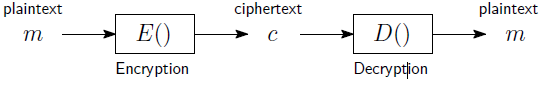
\includegraphics[height=7cm, width=9cm, keepaspectratio]{Immagini/introduzione/schema_blocchi_crittografia.png}}
	\caption{Schema a blocchi che illustra il processo cifratura-decifratura \label{fig:schema_blocchi_crittografia}} 	
\end{figure}

\subsubsection{Definizione formale di un sistema crittografico} Formalmente, un sistema crittografico è costituito da sette componenti (a volte alcune di queste sono assenti o coincidono):
\begin{itemize} 
  \item l'insieme dei possibili input (plaintext)
  \item l'insieme dei possibili output (ciphertex)
  \item l'insieme delle possibili chiavi di cifratura
  \item l'insieme delle possibili chiavi di decifratura
  \item la corrispondenza tra chiavi di cifratura e di decifratura
  \item l'algoritmo di cifratura da usare
  \item l'algoritmo di decifratura da usare
\end{itemize}

\subsubsection{Complessità computazionale} 
Uno schema crittografico, anche assumendo che sia privo di vulnerabilità intrinseche, può essere (quasi) sempre sottoposto ad attacchi a forza bruta. Affinché ciò possa avvenire è necessario disporre di un test affidabile che permetta di dire \textbf{se una chiave scelta a caso è quella corretta}; cioè, essere in grado di \textbf{riconoscere il testo in chiaro}. Se tale precondizione è verificata si può perseguire un approccio esaustivo in cui si tentano tutte le chiavi. Uno schema crittografico è allora tanto più sicuro quanto è maggiore il costo computazionale necessario a violarlo. Contemporaneamente deve garantire l'efficienza di cifratura/decifratura. Formalizzando, possiamo definire un sistema \textbf{computazionalmente sicuro} se il testo cifrato generato soddisfa \textbf{uno} dei seguenti requisiti:
\begin{itemize} 
  \item il costo per rendere inefficace il cifrario supera il valore dell'informazione cifrata
  \item il tempo richiesto per rendere inefficace il cifrario supera l'arco temporale in cui l'informazione ha una qualche utilità
\end{itemize}

Per capire l'importanza di tali definizioni si pensi al seguente esempio: anziché crittografare un'informazione in modo tale che sia necessario un anno (con determinate risorse di calcolo) per effettuare un attacco brute force esaustivo, potrebbe convenire utilizzare un cifrario computazionalmente più debole e cambiare la password ogni mese. \\

Tuttavia, stimare lo sforzo computazionale richiesto per effettuare con successo la crittoanalisi del testo cifrato è molto difficile. Il tempo richiesto per un approccio a forza bruta fornisce soltanto un limite superiore: è realistico solo se l'algoritmo non presenta delle debolezze intrinseche di tipo matematico; in questo caso si possono effettuare stime ragionevoli su tempi e costi. In un approccio a forza bruta mediamente si devono provare metà di tutte le possibili chiavi. Ovviamente in questo processo prende parte, come variabile fondamentale, la lunghezza della chiave. Alcuni schemi crittografici prevedono una chiave avente lunghezza variabile: aumentandola aumenta la sicurezza, ma diminuisce l'efficienza. Altri schemi stabiliscono a priori la lunghezza della chiave, se si desidera aumentarla è necessario sviluppare algoritmi simili che utilizzano chiavi di lunghezza diversa, oppure è possibile combinare in modo opportuno tali schemi ottenendo uno schema risultante con una chiave globale più lunga (attenzione al modo in cui si combinano!).

\subsubsection{Algoritmo pubblico o segreto?}
Come specificato nella sezione riguardante i principi della sicurezza informatica, ottenere la sicurezza attraverso la segretezza della metodologia di cifratura/decifratura (\textbf{security by obscurity}) è assolutamente da evitare. Questo perché:
\begin{itemize} 
  \item mantenere la segretezza è difficile, poiché le tecniche di reverse engineering permettono di risalire al codice
  \item è una strategia in chiara opposizione al \textbf{fundamental tenet of cryptography}
\end{itemize}
Oggigiorno, nelle applicazioni di uso civile/commerciale si usano schemi crittografici di dominio pubblico. La segretezza, laddove prevista, è conseguenza di altre cause (e.g. protezione del segreto industriale, contesti militari).

\subsection{Attacchi a sistemi crittografici}
Si possono distinguere \textbf{cinque categorie di attacchi} in base al tipo di informazioni in possesso dell'attaccante (di cui gli ultimi due meno frequenti):

\subsubsection{Solo testo cifrato (ciphertext only)}
L'attaccante conosce l'algoritmo di cifratura e dispone soltanto di una certa quantità di testo cifrato. Nell'ipotesi che non vi siano vulnerabilità intrinseche nello schema crittografico, l'attaccante può tentare un attacco forza bruta, a patto che disponga di un \textbf{test affidabile per il riconoscimento del testo in chiaro} e di \textbf{potenza di calcolo sufficiente} ad eseguire tutti i tentativi. L'attacco in questione:
\begin{enumerate}
  \item genera tutte le possibili chiavi di decifratura
  \item per ogni chiave decripta il testo cifrato
  \item verifica se il testo cifrato è un messaggio verosimile
\end{enumerate} 

Tale attacco è anche noto come \textbf{testo in chiaro riconoscibile (recognizable plaintext)}. Riguardo la riconoscibilità del testo in chiaro va osservato che, nel caso di messaggi testuali, è molto improbabile che una chiave di decifratura \textbf{errata} permetta di ottenere un messaggio \textbf{verosimile}. \\

\textbf{Esempio:} il messaggio $m$ è una frase di un qualche linguaggio naturale. Ipotizzando che i caratteri di $m$ siano codificati in ASCII a 8 bit e il testo cifrato $c$ abbia la stessa lunghezza di $m$ (quasi sempre è così). Siano:
\begin{itemize} 
  \item $t$: il numero di caratteri di $m$ e di $c$
  \item $n$ = $8t$: il numero di bit di $m$ e di $c$
  \item $2^{\alpha n}$: il numero totali di messaggi distinti, nel linguaggio naturale considerato, di lunghezza $n$ bit
\end{itemize}
Si osservi che nominalmente esistono $2^n$ stringhe binarie di $n$ bit, ma solo una piccolissima frazione di queste è la codifica di un messaggio nel linguaggio naturale, $0 < \alpha < 1$ è un fattore correttivo usato per modellare tale fenomeno, per la lingua inglese $\alpha = 0.16$.
\begin{figure}[htbp]
	\centering%
	\subfigure%
	{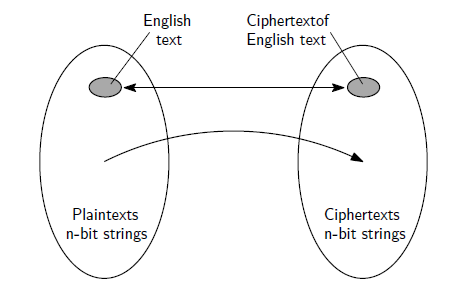
\includegraphics[height=8cm, width=8cm, keepaspectratio]{Immagini/introduzione/attacco_solo_tc.png}}
\end{figure}
\newline
Il seguente rapporto:
\begin{equation}
p_{v} = \frac{2^{\alpha n}}{2^n} = \frac{1}{2^{(1 - \alpha)n}}
\end{equation}
rappresenta la probabilità che un stringa random di $n$ bit costituisca la codifica di un messaggio nel linguaggio naturale considerato. Se la chiave di decifratura ha una lunghezza di $k$ bit, effettuando un attacco a forza bruta ($2^k$ tentativi), il numero atteso di messaggi verosimili (nel linguaggio naturale dato) associabili al testo cifrato $c$ è pari a:
\begin{equation}
numero \: tentativi  \cdot p_{v} = \frac{2^k}{2^{(1 - \alpha)n}}
\end{equation}
Essendo \textbf{k} fissato, al crescere di \textbf{n} tale numero tende rapidamente a zero, quindi il test di riconoscibilità diventa quasi infallibile se si dispone di una sufficiente quantità di testo cifrato. In alcuni casi, si potrebbe tentare un approccio a forza bruta computazionalmente meno costoso se:
\begin{itemize} 
  \item la chiave di decifratura coincide con quella di cifratura, spesso è così
  \item la chiave di cifratura è derivata da una password di utente segreta con una procedura nota (si può tentare un approccio a forza bruta sullo spazio delle password, sensibilmente più piccolo dello spazio delle chiavi)
\end{itemize}
\textbf{Uno schema crittografico deve \underline{sempre} essere sicuro contro attacchi di tipo ciphertext only, poiché il testo cifrato è sempre facilmente intercettabile e ottenibile.}

\subsubsection{Testo in chiaro conosciuto (known plaintext)}
In questo caso, il crittoanalista conosce:
\begin{itemize} 
  \item l'algoritmo di cifratura
  \item un certo insieme di coppie $\langle plaintext, ciphertext \rangle$, ma non ha la facoltà di decidere lui il tipo specifico di plaintext
  \item una certa quantità di testo cifrato
\end{itemize}
Alcuni schemi crittografici potrebbero essere molto resistenti ad attacchi di tipo \textbf{ciphertext only} ma rivelarsi vulnerabili ad attacchi di tipo \textbf{known plaintext}. In caso di impiego, è fondamentale prevenire che un attaccante ottenga coppie $\langle plaintext, ciphertext \rangle$.

\subsubsection{Testo in chiaro selezionato (chosen plaintext)}
In questo caso, il crittoanalista conosce:
\begin{itemize} 
  \item l'algoritmo di cifratura
  \item una certa quantità di testo cifrato (con chiave segreta K)
\end{itemize}
e può scegliere a piacimento il testo in chiaro ed ottenere il relativo testo cifrato (sempre con la chiave K). In altre parole può scegliere quali coppie $\langle plaintext, ciphertext \rangle$ conoscere. E' possibile che un sistema crittografico sia sicuro contro attacchi di tipo \textbf{ciphertext only} e \textbf{known plaintext}, ma sia vulnerabile ad attacchi di tipo \textbf{chosen plaintext}.

\subsubsection{Testo cifrato selezionato (chosen ciphertext)}
L'attaccante dispone (oltre che dell'algoritmo di cifratura e del testo cifrato da decifrare) di testo cifrato, con significato, scelto da lui, e corrispondente testo in chiaro.
\subsubsection{Testo selezionato (chosen text)}
L'attaccante dispone sia di testo in chiaro scelto da lui (e corrispondente testo cifrato) sia di testo cifrato scelto da lui (e corrispondente testo in chiaro).
\begin{figure}[htbp]
	\centering%
	\subfigure%
	{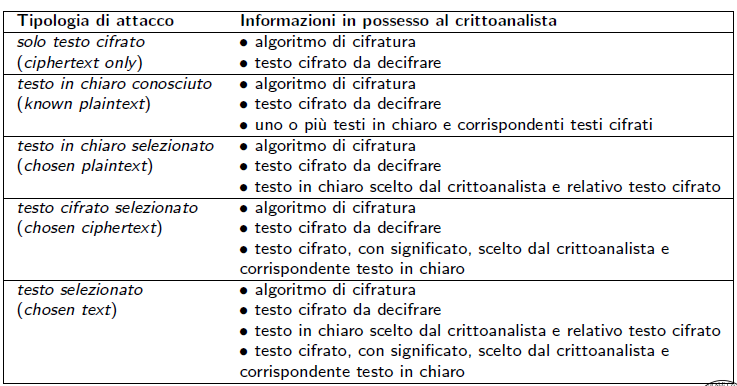
\includegraphics[height=12cm, width=13cm, keepaspectratio]{Immagini/introduzione/tab_attacchi_cifrari.png}}
	\caption{Tabella riassuntiva tipologie di attacchi \label{fig:tab_attacchi_cifrari}} 	
\end{figure}
\begin{figure}[htbp]
	\centering%
	\subfigure%
	{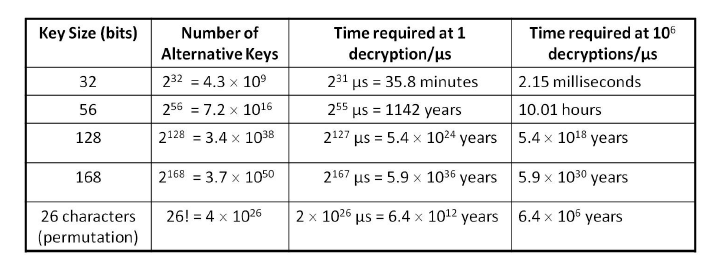
\includegraphics[height=12cm, width=13cm, keepaspectratio]{Immagini/introduzione/tab_tempi.png}}
	\caption{Tempo medio per una ricerca esaustiva \label{fig:tab_tempi}} 	
\end{figure}

\subsection{Tipi di funzioni crittografiche}
\begin{itemize} 
  \item funzioni a \textbf{chiave pubblica} (public key functions): richiedono l'uso di due chiavi, una pubblica e una privata (approfondire non ripudio su firma digitale). La crittografia a chiave pubblica è trattata nel Capitolo~\ref{ch:publickey}
  \item funzioni a \textbf{chiave segreta} (secret key functions): richiedono l'uso di una singola chiave. La crittografia a chiave segreta è trattata nel Capitolo~\ref{ch:secretkey}
  \item funzioni \textbf{hash} (hash functions): non usano alcuna chiave. Le funzioni crittografiche di hash sono trattate nel Capitolo~\ref{ch:hash}
\end{itemize}

\section{Modelli di controllo degli accessi (Access control models)}
Il controllo degli accessi alla varie risorse di un sistema informativo costituisce un fondamentale meccanismo di sicurezza di tipo \textbf{preventivo}. Previene attacchi alla confidenzialità, all'integrità e all'anonimato. L'idea di base è restringere l'accesso solo a coloro che hanno la necessità di accedere e/o modificare specifiche risorse, in accordo al principio del \textbf{minimo privilegio}.

\subsection{Matrice di controllo degli accessi} 
Una matrice di controllo degli accessi (Access Control Matrix ACM) è una tabella che definisce i permessi di accesso dei vari \textbf{soggetti} di un sistema informativo ai suoi \textbf{oggetti}.
\begin{itemize} 
  \item un \textbf{soggetto} è un utente, un gruppo o una generica entità attiva che desidera effettuare una data azione su un data risorsa
  \item un \textbf{oggetto} è un file, un documento, un dispositivo, una generica risorsa o più in generale un'entità passiva sulla quale si desidera compiere una data azione
\end{itemize}

Ogni riga della tabella è associata ad un soggetto, e ogni colonna è associata ad un oggetto. Ogni cella stabilisce quindi il tipo di azione consentita; il soggetto e l'oggetto sono implicitamente definiti dagli indici di riga e colonna della cella. Diverse modalità di accesso sono possibili: lettura, scrittura, copia, esecuzione, cancellazione, annotazione. Una cella vuota stabilisce che non viene assegnato alcun tipo di accesso.
\begin{figure}[htbp]
	\centering%
	\subfigure%
	{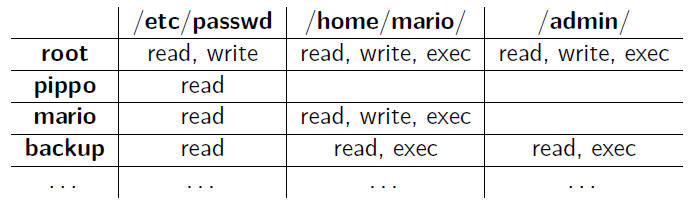
\includegraphics[height=11cm, width=11cm, keepaspectratio]{Immagini/introduzione/access_control_matrix_ex.png}}
	\caption{Esempio access control matrix \label{fig:acm}} 	
\end{figure}

\subsubsection{Pro e Contro ACM}
L'adozione di una ACM offre, in linea di principio, i seguenti vantaggi:
\begin{itemize} 
  \item immediatezza nel valutare e modificare i diritti di accesso per una data coppia soggetto-oggetto
  \item facilità di visualizzazione e gestione: semplifica la vita all'amministratore
\end{itemize}
Purtroppo, il grande svantaggio delle ACM, che ne limita fortemente l'applicabilità, è la mancanza di scalabilità. E' del tutto ragionevole pensare che un computer server possa avere ordine di $10^3$ soggetti (per lo più utenti) e $10^6$ oggetti (files e directories), richiedendo una ACM di $10^9$ celle. In questi ordini di grandezza i precedenti vantaggi decadono (\textbf{non scalabilità}).

\subsection{Liste di controllo degli accessi (Access Control List ACL)}
Una lista di controllo degli accessi (access control list ACL) segue un approccio di tipo \textbf{object-centered} per garantire una buona scalabilità, in particolare:
\begin{itemize} 
  \item ad ogni oggetto \textbf{o} viene associata un lista \textbf{L}, detta la lista di accesso di \textbf{o}, che enumera tutti i soggetti che hanno un qualche diritto di accesso ad \textbf{o}, e
  \item per ciascuno di tali soggetti \textbf{s} sono specificati i tipi di azioni che \textbf{s} può compiere su \textbf{o}
\end{itemize}
\begin{figure}[htbp]
	\centering%
	\subfigure%
	{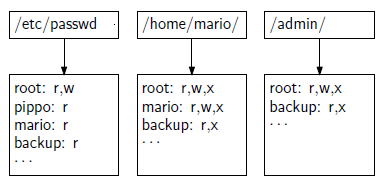
\includegraphics[height=8cm, width=8cm, keepaspectratio]{Immagini/introduzione/access_control_list_ex.png}}
	\caption{Esempio access control list \label{fig:acl}} 	
\end{figure}
Nella pratica, il modello ACL comporta un significativo risparmio di memoria rispetto al modello ACM: ogni lista del modello ACL è ottenibile scandendo la relativa colonna del modello ACM ignorando però le celle vuote.

\subsubsection{Pro e Contro ACL}
Il principale vantaggio del modello ACL rispetto al modello ACM è la \textbf{minor occupazione di memoria} che si registra nella pratica (in teoria, nel caso peggiore l'occupazione è la medesima). La memoria occupata complessivamente nel modello ACL, $\sum_{O} size(L_{O})$, è proporzionale a $C_{nv} (ACM)$ cioè al numero di celle non vuote della ACM. Nella pratica $C_{nv} (ACM)$ è molto minore di $C (ACM)$ (che denota il numero totale di celle della ACM) $\Rightarrow C_{nv} (ACM)<<C (ACM)$. \\
Un altro vantaggio è la facilità di gestione delle ACL da parte del sistema operativo:
\begin{itemize} 
  \item sono incorporate nei metadati associati all'oggetto in questione (i.e. filesystem)
  \item per verificare i diritti di accesso ad un oggetto \textbf{o} non è necessario consultare una struttura dati centralizzata associata a tutti gli oggetti
  \item ma basta manipolare una struttura dati molto più snella, distribuita ed associata soltanto all'oggetto \textbf{o}
\end{itemize}

Il principale svantaggio delle ACL è che non consente di enumerare in modo efficiente i diritti di accesso di un dato soggetto. Tale operazione deve essere espletata ogni qual volta un utente viene rimosso da un sistema. I diritti di accesso di un soggetto \textbf{s} possono ottenersi soltanto effettuando una scansione di tutte le liste di accesso (associate a tutti gli oggetti \textbf{o}), e selezionando i diritti di accesso di \textbf{s} nelle liste in cui tale soggetto compare. Nel modello ACM, invece, ciò poteva banalmente ottenersi esaminando la riga della matrice relativa al soggetto \textbf{s}.

\subsection{Controllo degli accessi basato su liste di capacità (Capabilities Access Control CAC)}
Il modello basato sulle liste di capacità segue un approccio \textbf{subject-centered}, complementare (ortogonale) a quello del modello ACL, per offrire una buona scalabilità. Ad ogni soggetto \textbf{s} viene associata una lista, detta \textbf{C-list} di \textbf{s}, contenente soltanto gli oggetti per i quali \textbf{s} ha un qualche diritto di accesso. Per ciascun oggetto \textbf{o} della \textbf{C-list} di \textbf{s} viene specificato il tipo di azione che \textbf{s} può esercitare su \textbf{o}. Similmente al modello ACL, anche il modello CAC comporta un significativo risparmio di memoria rispetto al modello ACM nelle situazioni pratiche: ogni lista del modello CAC è ottenibile scandendo la relativa riga del modello ACM ignorando però le celle vuote. 
\begin{figure}[htbp]
	\centering%
	\subfigure%
	{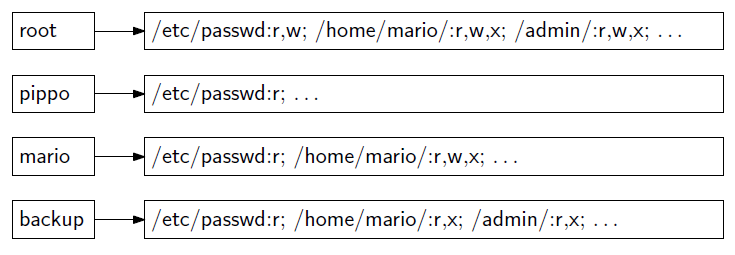
\includegraphics[height=10cm, width=10cm, keepaspectratio]{Immagini/introduzione/CAC_ex.png}}
	\caption{Esempio CAC \label{fig:CAC}} 	
\end{figure}
\subsubsection{Pro e Contro CAC}
Rispetto al modello ACM, anche il modello CAC richiede una minor occupazione di memoria nella pratica. La memoria occupata complessivamente nel modello CAC,  $\sum_{s} size(L_{s})$, è proporzionale a $C_{nv} (ACM)$, cioè al numero di celle non vuote della ACM (vedi considerazioni su ACL). Facilita inoltre il compito dell'amministratore di sistema nell'analizzare e gestire i diritti di accesso di un dato soggetto. Inoltre, l'autorizzazione ad accedere ad un dato oggetto o da parte di un soggetto \textbf{s} richiede tempi ragionevolmente brevi qualora la \textbf{C-list} di \textbf{s} abbia una dimensione contenuta.\newline \newline
Il principale svantaggio del modello CAC è che le \textbf{C-list} non sono direttamente associate agli oggetti. Ciò comporta che:
\begin{itemize} 
  \item non è possibile implementarle in modo distribuito incorporandole nei metadati degli oggetti
  \item l'unico modo per determinare chi e come può accedere ad un dato oggetto o è effettuare una ricerca su tutte le C-list (di tutti i soggetti); nel modello ACM tale operazione richiede semplicemente di esaminare la colonna relativa ad o (problema ortogonale a quello delle ACL)
\end{itemize}

\subsection{Controllo degli accessi basato sui ruoli (Role-Based Access Control RBAC)}
Per controllo degli accessi basato sui ruoli si intende che l'assegnazione dei diritti di accesso avviene in modo indiretto ed è funzione del ruolo attribuito ad un dato soggetto \textbf{s}. L'amministratore definisce i ruoli e specifica i diritti di accesso per tali ruoli, anziché quelli per i singoli soggetti (utenti). Ogni ruolo dovrebbe rappresentare una classe di soggetti (utenti) con la medesima mansione. I soggetti vanno assegnati ai vari ruoli coerentemente alle loro mansioni, e un soggetto può ricevere più ruoli dato che può ricoprire più mansioni. Definiti i ruoli, i diritti di accesso vanno assegnati secondo una logica ruolo-oggetto e NON soggetto-oggetto. I diritti di accesso di un dato soggetto sono l'unione dei diritti di accesso dei suoi ruoli. Pertanto:
\begin{itemize} 
  \item \textbf{il modello RBAC non è alternativo ai modelli ACM, ACL e CAC, ma si pone ad un livello di astrazione superiore}: RBAC deve necessariamente sfruttare un modello per il controllo degli accessi, basato su \textbf{ACM}, \textbf{ACL} o \textbf{CAC}, ove i soggetti saranno però sostituiti dai ruoli.
  \item RBAC deve inoltre mantenere/gestire l'elenco dei ruoli associati ai vari soggetti
\end{itemize}

\subsubsection{Architettura RBAC}
Il modello RBAC è realizzabile utilizzando un generico framework per la gestione del controllo degli accessi (ACM, ACL, CAC), ove i soggetti sono, come già detto, sostituiti con i ruoli, più un layer superiore che gestisce l'elenco dei ruoli associati ai vari soggetti e che traduce le richieste di accesso per un dato soggetto in quelle relative ai suoi ruoli.
\begin{figure}[htbp]
	\centering%
	\subfigure%
	{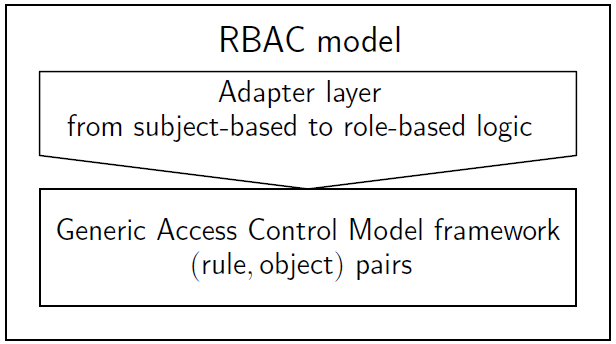
\includegraphics[height=10cm, width=10cm, keepaspectratio]{Immagini/introduzione/RBAC_arch.png}}
	\caption{Architettura RBAC \label{fig:RBAC_arch}} 	
\end{figure}

\subsubsection{Gerarchia dei ruoli}
Generalmente è conveniente organizzare i ruoli in una struttura gerarchica, così da riflettere l'organigramma (gerarchico) di una data organizzazione. I diritti di accesso vengono più agevolmente gestiti e assegnati ai vari ruoli sfruttando l'ereditarietà.
\begin{figure}[htbp]
	\centering%
	\subfigure%
	{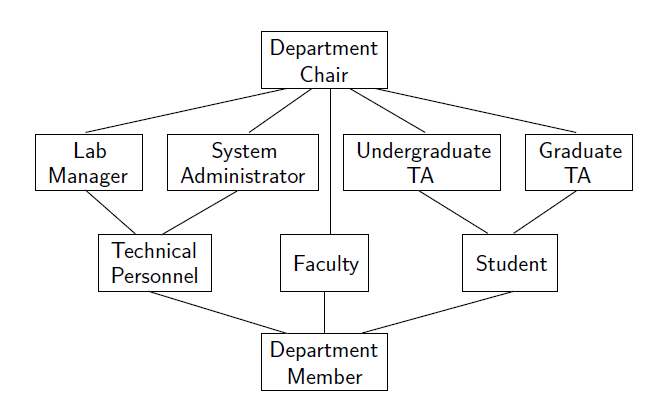
\includegraphics[height=7cm, width=7cm, keepaspectratio]{Immagini/introduzione/RBAC_ger.png}}
	\caption{Architettura RBAC \label{fig:RBAC_ger}} 	
\end{figure}

\subsubsection{Pro e Contro RBAC}
Indipendentemente dal framework di basso di livello utilizzato per il controllo degli accessi, i vantaggi nell'uso del modello RBAC sono:
\begin{itemize} 
  \item la riduzione drastica del numero totale di regole di accesso da gestire: nella pratica il numero dei ruoli è significativamente inferiore a quello dei soggetti, inoltre la loro organizzazione gerarchica ne semplifica ulteriormente la gestione.
  \item l'overhead per determinare se un dato soggetto ha un dato diritto è contenuto: è sufficiente consultare se almeno uno dei suoi ruoli ha tale diritto.
\end{itemize}
Lo svantaggio principale è che non viene implementato dagli attuali sistemi operativi!
